\documentclass[12pt,a4paper]{article}
\usepackage[utf8]{inputenc}
\usepackage[spanish,es-tabla,es-noquoting]{babel}
\usepackage{geometry}
\usepackage{graphicx}
\usepackage{multirow}
\usepackage{tabularx}
\usepackage{longtable}
\usepackage{float}
\usepackage{amsmath}
\usepackage{amssymb}
\usepackage{mathptmx}
\usepackage{fancyhdr}
\usepackage{array}
\usepackage[table]{xcolor}
\usepackage{titlesec}
\usepackage{setspace}
\usepackage{microtype}
\usepackage{lastpage}
\usepackage{booktabs}
\usepackage{enumitem}
\usepackage{hyperref}
\usepackage{listings}

\hypersetup{
    colorlinks=true,
    linkcolor=black,
    citecolor=blue!70!black,
    urlcolor=blue!70!black
}

\graphicspath{{images/}{../images/}{./}}

\geometry{
    top=4.7cm,
    bottom=2.5cm,
    left=2.5cm,
    right=2.5cm,
    headheight=3.9cm,
    headsep=0.4cm
}

\setstretch{1.15}
\setlength{\parindent}{0pt}
\setlength{\parskip}{0.45em}
\setlength{\tabcolsep}{4pt}

\titleformat{\section}
  {\normalfont\fontsize{12}{14.5}\bfseries}{\thesection.}{0.6em}{\uppercase}
\titlespacing*{\section}
  {0pt}{1.8ex plus 0.4ex minus 0.2ex}{0.6ex plus 0.2ex}

\titleformat{\subsection}
  {\normalfont\fontsize{11.5}{13.5}\bfseries}{\thesubsection.}{0.5em}{}
\titlespacing*{\subsection}
  {0pt}{1.4ex plus 0.3ex minus 0.1ex}{0.4ex plus 0.1ex}

\titleformat{\subsubsection}
  {\normalfont\fontsize{10.5}{12.5}\bfseries\itshape}{\thesubsubsection.}{0.4em}{}
\titlespacing*{\subsubsection}
  {0pt}{1.1ex plus 0.2ex minus 0.1ex}{0.3ex plus 0.1ex}

\newcolumntype{Y}{>{\centering\arraybackslash}X}
\newcolumntype{L}{>{\raggedright\arraybackslash}X}
\newcolumntype{C}{>{\centering\arraybackslash}X}

\definecolor{headerred}{RGB}{180, 0, 0}
\definecolor{darkred}{RGB}{140, 0, 0}
\definecolor{lightgraybg}{RGB}{248, 248, 248}
\definecolor{tableheader}{RGB}{232, 238, 246}
\definecolor{navyheader}{RGB}{0, 52, 94}

\newcommand{\docCodigo}{TI-SIGE-ENT-F3-013}
\newcommand{\docVersion}{1.0}
\newcommand{\docProceso}{INGENIERÍA DE SOFTWARE / MODELOS DE LENGUAJE LOCALES}
\newcommand{\docElaboracion}{07/10/2026}
\newcommand{\docRevision}{07/10/2026}
\newcommand{\docTitulo}{INTEGRACIÓN DE CAPA DE IA LOCAL: ASISTENCIA SEMÁNTICA CON OLLAMA LLM}
\newcommand{\docOrganizacion}{FACULTAD DE INGENIERÍA EN SISTEMAS, ELECTRÓNICA E INDUSTRIAL}
\newcommand{\docSubOrganizacion}{CARRERA DE INGENIERÍA DE SOFTWARE}

\newcommand{\encabezadofrecuente}{%
    \renewcommand{\arraystretch}{1.15}%
    \noindent\makebox[\textwidth][c]{%
    \begin{tabularx}{\textwidth}{|>{\centering\arraybackslash}m{2.8cm}|Y|>{\centering\arraybackslash}m{4.8cm}|}
        \hline
        \multirow{4}{2.8cm}{\centering\raisebox{-1.15cm}{
\includegraphics[width=2.5cm,height=2.0cm,keepaspectratio]{images/logo.png}}}
        & \textbf{\fontsize{9}{11}\selectfont \docOrganizacion} 
        & \textbf{\fontsize{8}{10}\selectfont CÓDIGO:} \fontsize{8}{10}\selectfont \docCodigo \\
        \cline{3-3}
        & \textbf{\fontsize{8.5}{10.5}\selectfont \docSubOrganizacion} 
        & \textbf{\fontsize{8}{10}\selectfont VERSIÓN:} \fontsize{8}{10}\selectfont \docVersion \\
        \cline{2-3}
        & \textbf{\fontsize{8}{10}\selectfont PROCESO:} \fontsize{8}{10}\selectfont \docProceso 
        & \textbf{\fontsize{8}{10}\selectfont ELABORACIÓN:} \fontsize{8}{10}\selectfont \docElaboracion \\
        \cline{2-3}
        & \textbf{\fontsize{8.5}{10.5}\selectfont \docTitulo} 
        & \textbf{\fontsize{8}{10}\selectfont ÚLTIMA REVISIÓN:} \fontsize{8}{10}\selectfont \docRevision \\
        \hline
    \end{tabularx}%
    }%
}

\pagestyle{fancy}
\fancyhf{}
\fancyhead[C]{\encabezadofrecuente}
\fancyfoot[C]{\fontsize{10}{12}\selectfont Página \thepage\ de \pageref{LastPage}}
\renewcommand{\headrulewidth}{0pt}

\lstset{
  basicstyle=\ttfamily\scriptsize,
  backgroundcolor=\color{lightgraybg},
  frame=single,
  breaklines=true,
  tabsize=2,
  showstringspaces=false
}

\begin{document}

\noindent{\fontsize{10.5}{12.5}\selectfont \textbf{Integrantes:} Heidi Villavicencio \quad$\vert$\quad Steeven Toala \quad$\vert$\quad Nixon Hurtado \quad$\vert$\quad Andrea Vásquez}

\vspace{0.25cm}

\section{Título}
\textbf{Denominación del Entregable:} Integración de la Capa de Inteligencia Local: Asistente Semántico con Ollama LLM para Formulación de Objetivos y Síntesis Académica -- Código EDT: 3.13 (Fase 3: Desarrollo Iterativo Core).

\section{Introducción}
La redacción de los Planes de Trabajo Docente y los Informes Semestrales en la FISEI exige coherencia pedagógica entre las asignaturas impartidas, las horas asignadas y los objetivos de aprendizaje formulados según la Taxonomía de Bloom. Los docentes frecuentemente se enfrentan a dificultades para sintetizar logros académicos o redactar justificaciones claras bajo la terminología requerida por el Sistema de Gestión de Calidad (SGC).

El uso de servicios de inteligencia artificial comerciales en la nube (como OpenAI o Anthropic) presenta serios riesgos de privacidad y fuga de información académica protegida por la Ley Orgánica de Protección de Datos Personales (LOPDP) de Ecuador y la normativa de seguridad de la información ISO/IEC 27001. En consecuencia, el proyecto SIGE adopta una arquitectura de \textbf{IA Local Soberana} mediante el motor \textbf{Ollama}, ejecutando modelos de lenguaje de gran escala (LLM) de parámetros abiertos en el entorno institucional sin conexión a internet ni costos por consumo de tokens externos.

\section{Objetivo}

\subsection{Objetivo General}
Implementar un servicio de asistencia semántica basado en un modelo LLM local orquestado mediante Ollama, integrado de forma segura y supervisada en la plataforma SIGE para apoyar al cuerpo docente en la formulación de objetivos y redacción de informes.

\subsection{Objetivos Específicos}
\begin{itemize}[leftmargin=1.5em, itemsep=1.5pt]
    \item Integrar el motor Ollama en la infraestructura local con un modelo optimizado en español (Llama 3 8B / Mistral 7B cuantizado a Q4).
    \item Diseñar plantillas de ingeniería de prompts (\textit{Prompt Engineering}) restringidas al dominio del SGC de la UTA y verbos de Bloom.
    \item Implementar el puente de conexión asíncrono en Express con streaming de respuestas y control de latencia.
\end{itemize}

\section{Alcance}

\subsection{Límites de Implementación (In-Scope)}
\begin{itemize}[leftmargin=1.5em, itemsep=1.5pt]
    \item Sugerencia de objetivos específicos a partir del nombre de la materia y la justificación redactada por el docente.
    \item Resumen y síntesis ejecutiva de las actividades cumplidas para la sección de Conclusiones del informe.
    \item Modo de operación 100\% asistido: el docente tiene el control total para aceptar, editar o descartar las sugerencias.
\end{itemize}

\subsection{Exclusiones (Out-of-Scope)}
\begin{itemize}[leftmargin=1.5em, itemsep=1.5pt]
    \item Creación automatizada o ficticia de actividades sin aprobación explícita del docente.
    \item Aprobación autónoma de informes por parte del modelo de lenguaje.
\end{itemize}

\section{Definiciones}
\begin{itemize}[leftmargin=1.5em, itemsep=2pt]
    \item \textbf{Ollama:} Entorno de ejecución ligero para ejecutar modelos de lenguaje grandes (LLMs) localmente en hardware institucional.
    \item \textbf{Cuantización (Q4\_K\_M):} Técnica de compresión de pesos del modelo a 4 bits que reduce el consumo de memoria RAM/VRAM en más del 70\% manteniendo la precisión lingüística.
    \item \textbf{Taxonomía de Bloom:} Clasificación pedagógica de objetivos educativos organizada en niveles de dominio cognitivo (Recordar, Comprender, Aplicar, Analizar, Evaluar, Crear).
    \item \textbf{Prompt del Sistema (System Prompt):} Conjunto de directrices rígidas iniciales que instruyen al modelo a actuar exclusivamente como un asistente académico de la FISEI UTA.
\end{itemize}

\section{Responsabilidades}
\begin{itemize}[leftmargin=1.5em, itemsep=2pt]
    \item \textbf{Analista de Requisitos / UI-UX (Heidi Villavicencio):} Relevamiento y modelado de necesidades, especificaciones funcionales, diseño de interfaces de usuario y verificación de usabilidad.
    \item \textbf{Líder de Proyecto / Arquitecto de Software (Steeven Toala):} Arquitectura de software, gobierno técnico, cumplimiento metodológico del cronograma y control de calidad integral.
    \item \textbf{Desarrollador Backend / DBA (Nixon Hurtado):} Modelo de base de datos PostgreSQL, persistencia de datos, seguridad por roles y reglas lógicas de validación.
    \item \textbf{Desarrolladora Frontend / QA (Andrea Vásquez):} Implementación de componentes React, manejo de estado global, integración de APIs y ejecución de pruebas de aceptación.
    \item \textbf{Docente Evaluador / Tutor (Ing. Paulo Torres, Mg.):} Dirección académica, asesoría metodológica, revisión de suficiencia técnica y validación institucional de los entregables.
\end{itemize}

\section{Normativa Legal y Técnica}
\begin{itemize}[leftmargin=1.5em, itemsep=2pt]
    \item \textbf{ISO/IEC 27001:2022 (Privacidad y Aislamiento):} Garantía de que ninguna evidencia documental o dato sensible es transmitido a servidores externos.
    \item \textbf{Ley Orgánica de Protección de Datos Personales (Ecuador):} Principio de finalidad y proporcionalidad en el tratamiento de textos académicos.
    \item \textbf{UNESCO (Recomendación sobre la Ética de la Inteligencia Artificial):} Transparencia, supervisión humana y uso ético de modelos generativos en la educación superior.
\end{itemize}

\section{Método, Políticas y Contenidos}
Se adoptaron tres políticas estrictas de gobernanza para el asistente inteligente:
\begin{enumerate}[leftmargin=1.5em, itemsep=2pt]
    \item \textbf{Transparencia de Inferencia:} La interfaz indica con un badge visual cuando una sugerencia ha sido generada con soporte de IA.
    \item \textbf{Supervisión Humana Obligatoria (Human-in-the-Loop):} Ningún texto generado por el LLM se guarda en el borrador oficial sin la confirmación interactiva del docente.
    \item \textbf{Temperatura Determinística Reducida ($\mathbf{T = 0.2}$):} Se ajusta el parámetro de aleatoriedad del modelo a un valor bajo para evitar alucinaciones y favorecer respuestas sobrias y formales.
\end{enumerate}

\begin{figure}[htbp]
    \centering
    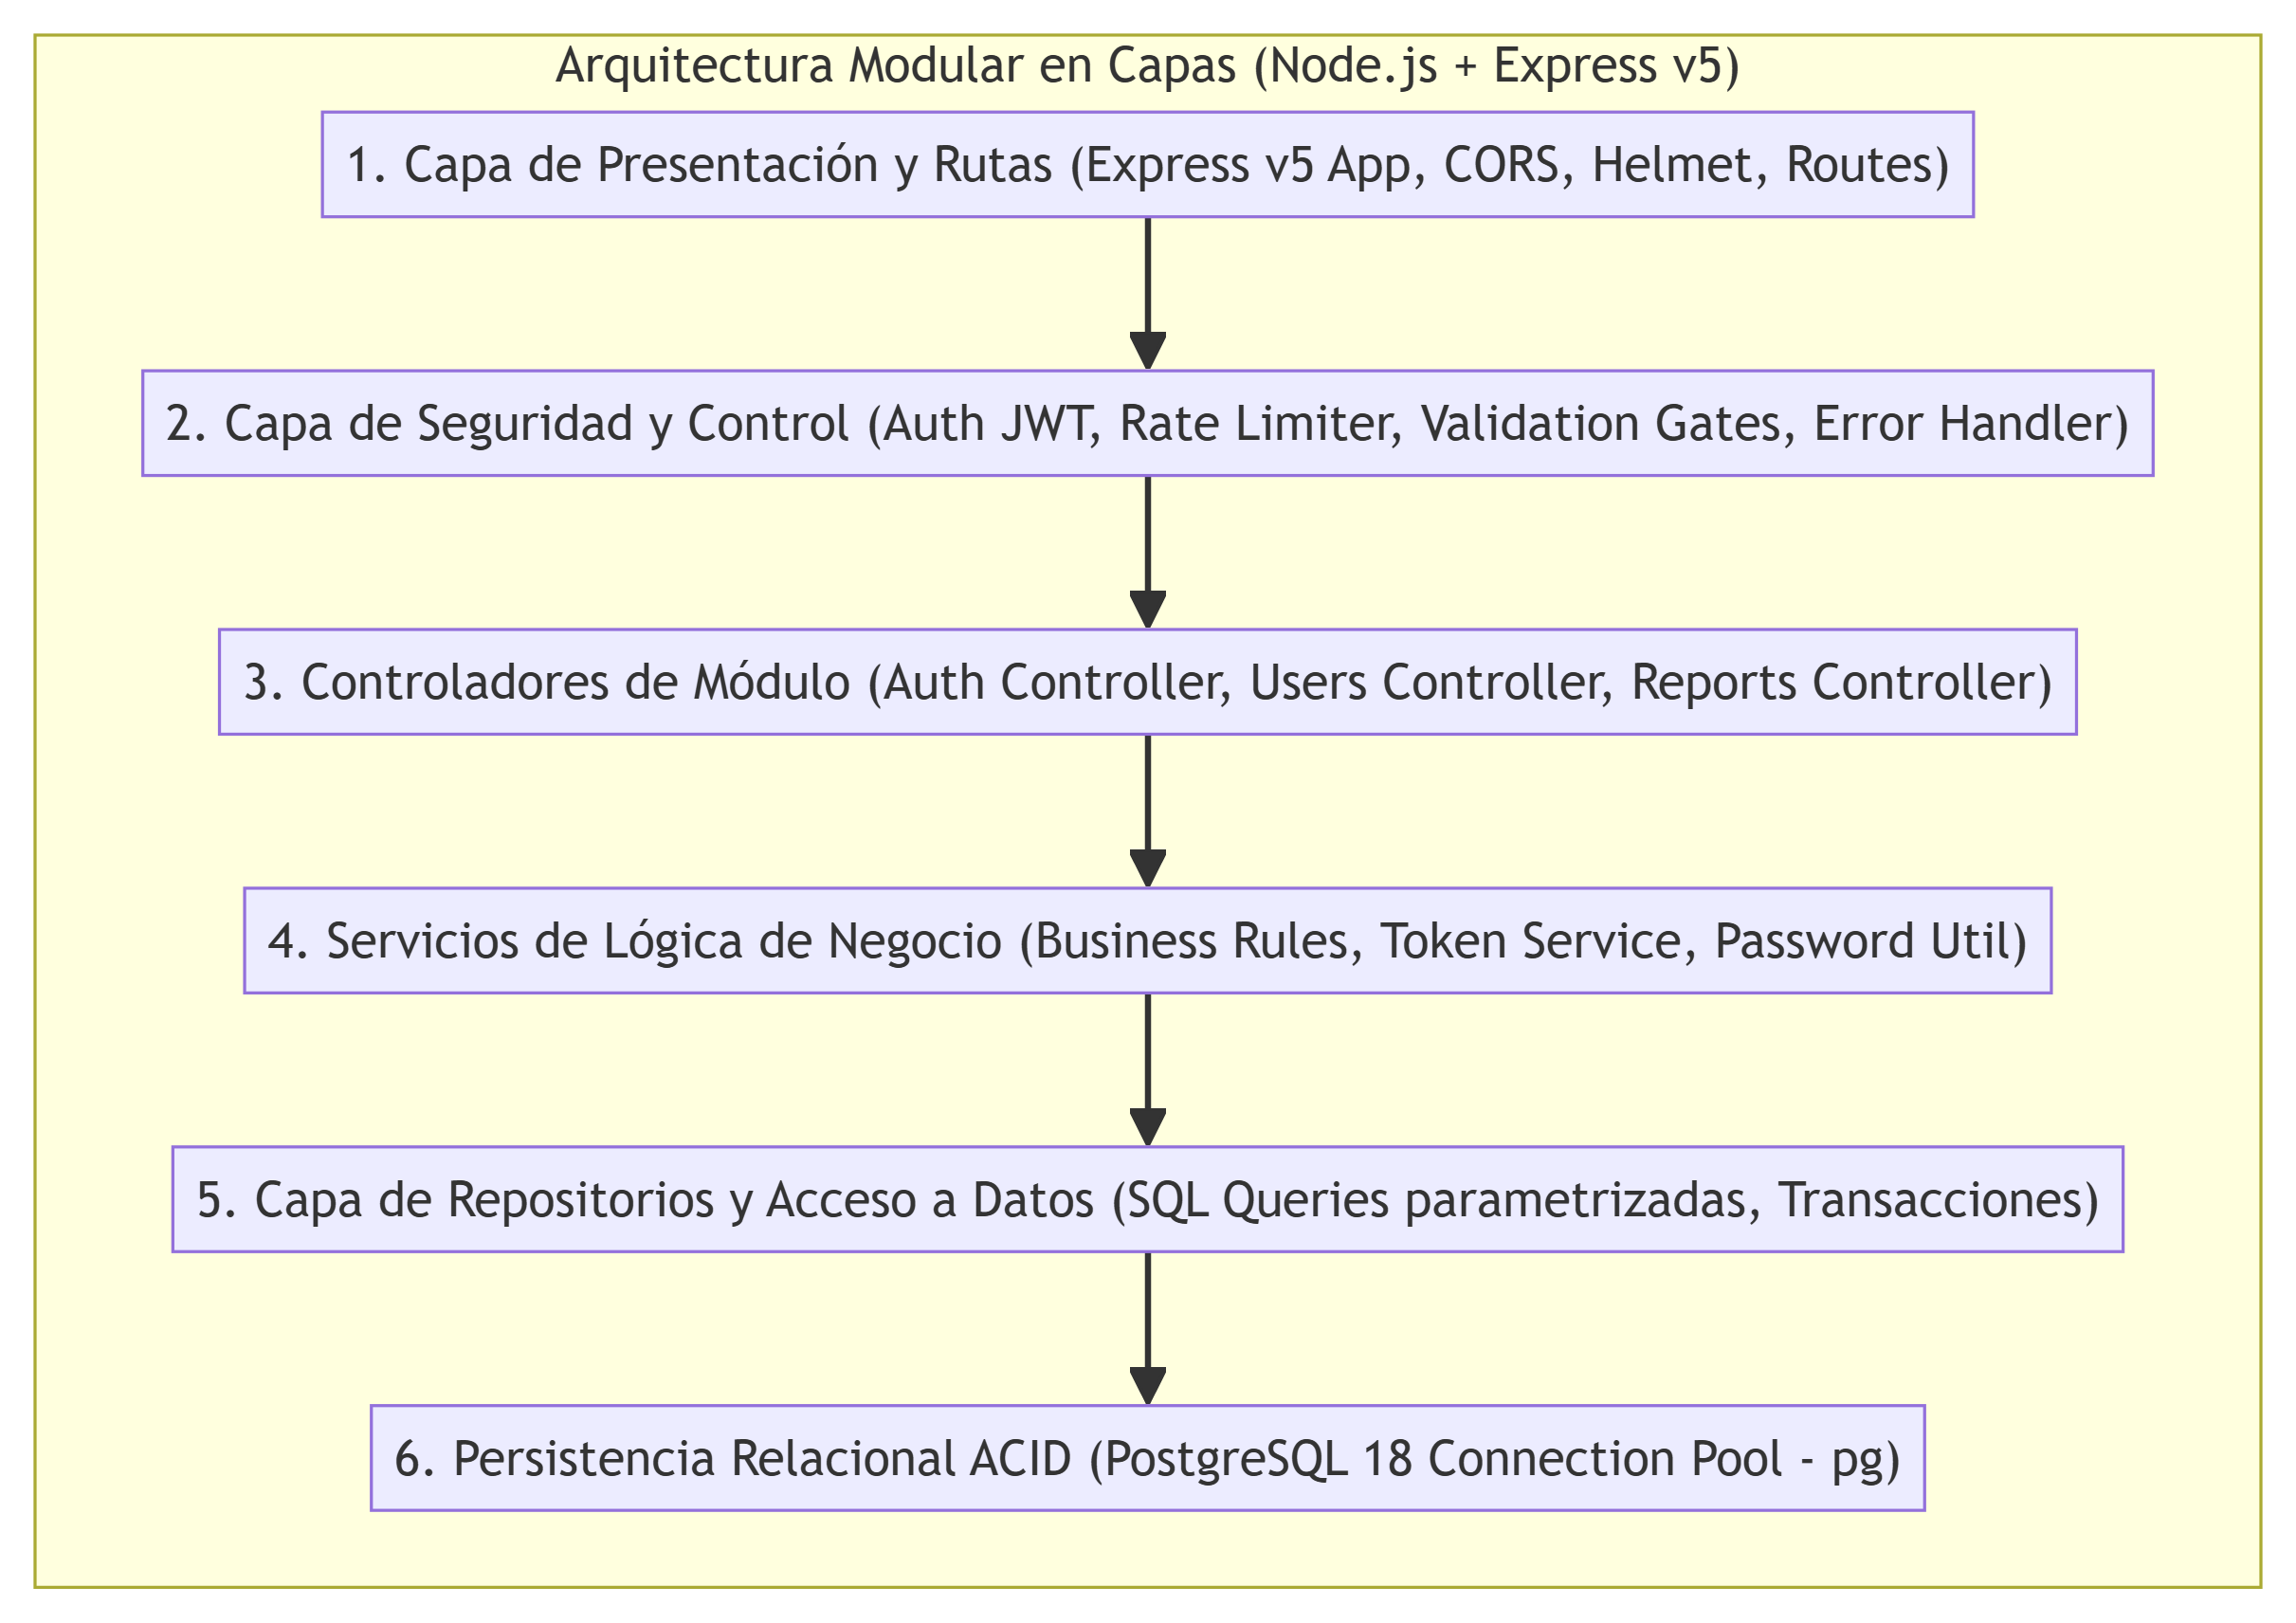
\includegraphics[width=0.88\textwidth,keepaspectratio]{images/s2_02_clean_architecture.png}
    \caption{Integración Desacoplada de la Capa de Inteligencia Local en la Arquitectura de SIGE.}
    \label{fig:arquitectura_ia}
\end{figure}

\section{Descripción de actividades}

\subsection{Plantilla de Ingeniería de Prompts (Prompt Template)}
Se diseñó un \textit{System Prompt} contextualizado para el reglamento institucional:
\begin{lstlisting}
Eres el Asistente Académico del Sistema SIGE de la FISEI - Universidad Técnica de Ambato.
Tu misión es asistir a los docentes en la redacción formal de Objetivos y Justificaciones.
Reglas:
1. Responde exclusivamente en español formal y académico.
2. Los objetivos deben iniciar con un verbo en infinitivo según la Taxonomía de Bloom.
3. No inventes asignaturas ni horas que no hayan sido provistas en el contexto.
4. Mantén tus respuestas concisas (máximo 3 párrafos o viñetas numeradas).
\end{lstlisting}

\subsection{Servicio de Integración en Backend (ollama.service.js)}
\begin{lstlisting}[language=JavaScript]
// backend/src/services/ollama.service.js
const axios = require('axios');

const OLLAMA_HOST = process.env.OLLAMA_HOST || 'http://localhost:11434';
const MODEL_NAME = process.env.OLLAMA_MODEL || 'llama3:8b-instruct-q4_K_M';

exports.generarSugerenciaObjetivos = async (asignatura, justificacion) => {
  const prompt = `Asignatura: ${asignatura}. Justificación: ${justificacion}.
Sugiere 3 objetivos específicos acordes a la carrera de Ingeniería de Software.`;

  const response = await axios.post(`${OLLAMA_HOST}/api/generate`, {
    model: MODEL_NAME,
    prompt: prompt,
    stream: false,
    options: {
      temperature: 0.2,
      top_p: 0.9,
      num_ctx: 2048
    }
  }, { timeout: 15000 });

  return response.data.response;
};
\end{lstlisting}

\begin{figure}[htbp]
    \centering
    
\includegraphics[width=0.88\textwidth,keepaspectratio]{images/plan_page_2.png}
    \caption{Asistente de Objetivos Académicos en el Formulario del Asistente Wizard de SIGE.}
    \label{fig:ollama_preview}
\end{figure}

\section{Firmas de Responsabilidad}

\noindent
\renewcommand{\arraystretch}{1.2}
\begin{tabularx}{\textwidth}{|>{\raggedright\arraybackslash}m{2.9cm}|>{\raggedright\arraybackslash}X|>{\centering\arraybackslash}m{4.6cm}|>{\centering\arraybackslash}m{2.3cm}|}
    \hline
    \rowcolor{tableheader}
    \textbf{ACCIÓN} & \textbf{NOMBRE Y CARGO} & \textbf{FIRMA} & \textbf{FECHA} \\
    \hline
    \textbf{Elaborado por:} & Heidi Villavicencio\newline Analista de Requisitos / UI-UX & \parbox[c]{4.4cm}{\centering\vspace{4pt}
\includegraphics[height=1.5cm,width=4.0cm,keepaspectratio]{images/firma_heidi.png}\vspace{4pt}} & 07/10/2026 \\
    \hline
    \textbf{Revisado por:} & Steeven Toala\newline Líder de Proyecto / Arquitecto & \parbox[c]{4.4cm}{\centering\vspace{4pt}
\includegraphics[height=1.5cm,width=4.0cm,keepaspectratio]{images/firma_steveen.png}\vspace{4pt}} & 07/10/2026 \\
    \hline
    \textbf{Revisado por:} & Nixon Hurtado\newline Desarrollador Backend / DBA & \parbox[c]{4.4cm}{\centering\vspace{8pt}\textbf{[ FIRMADO ELECTRÓNICAMENTE ]}\vspace{8pt}} & 07/10/2026 \\
    \hline
    \textbf{Revisado por:} & Andrea Vásquez\newline Desarrolladora Frontend / QA & \parbox[c]{4.4cm}{\centering\vspace{8pt}\textbf{[ FIRMADO ELECTRÓNICAMENTE ]}\vspace{8pt}} & 07/10/2026 \\
    \hline
    \textbf{Aprobado por:} & Ing. Paulo Torres, Mg.\newline Docente Evaluador -- Gestión Proyectos & \parbox[c]{4.4cm}{\centering\vspace{8pt}\textbf{\textcolor{gray!80}{\scriptsize [ PENDIENTE DE APROBACIÓN ]}}\vspace{8pt}} & \textbf{\textcolor{gray!90}{Pendiente}} \\
    \hline
\end{tabularx}

\vspace{0.4cm}

\section{Control de Cambios}

\noindent
\renewcommand{\arraystretch}{1.2}
\begin{tabularx}{\textwidth}{|>{\hsize=0.45\hsize\centering\arraybackslash}X|>{\hsize=1.55\hsize\raggedright\arraybackslash}X|>{\hsize=1.2\hsize\raggedright\arraybackslash}X|>{\hsize=0.8\hsize\centering\arraybackslash}X|}
    \hline
    \rowcolor{tableheader}
    \textbf{Versión} & \textbf{Descripción del cambio} & \textbf{Responsable del cambio} & \textbf{Fecha de aprobación} \\
    \hline
    1.0 & Integración del motor local Ollama con Llama 3 para sugerencias pedagógicas y redacción asistida. & Steeven Toala / Heidi Villavicencio & 07/10/2026 \\
    \hline
\end{tabularx}

\vspace{0.4cm}

\section{Anexos}

\subsection*{Anexo 1: Evaluación de Rendimiento del Modelo Ollama en Hardware Local}
\begin{table}[H]
\centering
\small
\begin{tabularx}{\textwidth}{|l|c|c|X|}
\hline
\rowcolor{tableheader}
\textbf{Modelo Cuantizado} & \textbf{RAM Requerida} & \textbf{Tokens / Seg} & \textbf{Consistencia Sintáctica SGC} \\ \hline
Llama 3 8B (Q4\_K\_M) & 4.8 GB & 24.5 tok/s & Alta (Adhesión estricta a verbos de Bloom) \\ \hline
Mistral 7B (Q4\_K\_M) & 4.1 GB & 28.2 tok/s & Media-Alta (Buena síntesis pero requiere afinar prompt) \\ \hline
Phi-3 Mini 3.8B (Q4) & 2.4 GB & 42.0 tok/s & Media (Respuestas breves; ideal para máquinas de bajo recurso) \\ \hline
\end{tabularx}
\caption{Comparativa de Modelos Locales Evaluados para el Servicio Ollama en SIGE.}
\label{tab:evaluacion_llm}
\end{table}

\end{document}
